\section{Gradient vs d-operator}

This sections explains the difference between these two operators, which many times can be confused.
And even though they're technically different things, they're highly related to each other.\\

First of all, we're going to call the operator:

\begin{itemize}
    \item $\grad{f}$ \text{the gradient of the scalar field f}
    \item $df$ \text{the differential of f, also known as the exterior derivative of f}
\end{itemize}

Both the gradient and the differential, act on a scalar field.\\
The gradient of the scalar field gives us a vector field, where the vectors point in the direction
of steepest increase, and larger vectors indicating a steeper change, whereas $df$ gives us a covector field, 
(also called 1-form), where the covector curves are given by the level sets of the scalar field.
And the level sets are oriented towards the positive values of the field.\\
So it's clear that the two are different, but at the same time fairly similar and highly related. 

\begin{center}
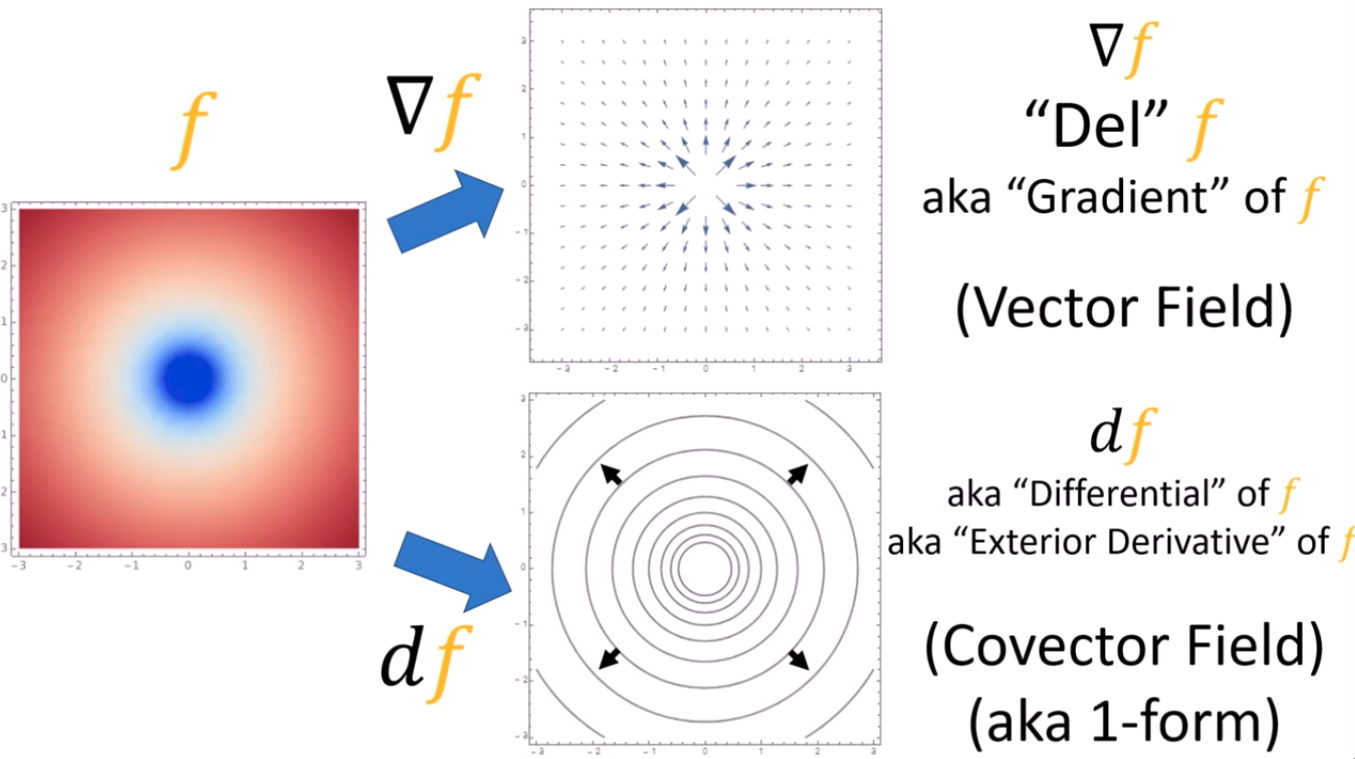
\includegraphics[scale=0.3]{figures/gradient-vs-d.png}
\end{center}

We know that there's a special connection between a vector space and its dual, and this special connection is given by 
pairing up a vector $\color{orange}\vec{v}$ with its dual partner covector $\begingroup\color{orange}\vec{v}\endgroup \cdot {{} - {}}$ and we 
saw this in our notes on raising/lowering indexes.\\
The connection between the two partners is possible via the metric tensor.\\
A similar pairing is actually possible between $\grad{\begingroup\color{orange}f\endgroup}$ and $d{\begingroup\color{orange}f\endgroup}$.\\

Let's recall that $d{\begingroup\color{orange}f\endgroup} (\begingroup\color{teal}\vec{v}\endgroup)$ is the directional 
derivative of $\begingroup\color{orange}f\endgroup$ in direction $\begingroup\color{teal}\vec{v}\endgroup$ and we can write:

\begin{equation}
    d{\begingroup\color{orange}f\endgroup} (\begingroup\color{teal}\vec{v}\endgroup) = \grad_{\begingroup\color{teal}\vec{v}\endgroup}{\begingroup\color{orange}f\endgroup}
    = \grad{\begingroup\color{orange}f\endgroup} \cdot \begingroup\color{teal}\vec{v}\endgroup
\end{equation}

This is already interesting, on the left we have the differential acting on a vector, and on the right we have the dot product 
of the gradient per the same vector.\\

In a sense, this means that $d{\begingroup\color{orange}f\endgroup} = \grad{\begingroup\color{orange}f\endgroup} \cdot {{} - {}}$.\\

Now, remember that from the raising/lowering indexes notes, we know that:

\begin{equation}
    \begingroup\color{orange}\vec{v}\endgroup \cdot  {{} - {}} = \begingroup\color{orange}v^i\endgroup \begingroup\color{cyan}g_{ij}\endgroup \begingroup\color{blue}\epsilon^i\endgroup
\end{equation}

And:

\begin{center}
\begin{tikzpicture}[
    box/.style={draw, thick, minimum width=4cm, minimum height=6cm},
    every node/.style={font=\Large}
]

% Left box (V)
\node[box] (V) at (0,0) {};
\node at (V.north) [below=1cm] {$V$};

% Circled v in left box
\node at (V.south) [above=1.2cm] 
{
    \tikz{
        \node[draw, circle, thick, inner sep=6pt] 
        {$\color{orange}{\vec{v}}$};
    }
};

% Arrow with g
\draw[thick, ->] (2.8,1) -- (6.2,1)
    node[midway, above=2pt] {$g$};

% Arrow with g-inverse
\draw[thick, <-] (2.8,-1) -- (6.2,-1)
    node[midway, below=2pt] {$\mathfrak{g}$};


% Right box (V*)
\node[box] (Vstar) at (9,0) {};
\node at (Vstar.north) [below=1cm] {$V^{*}$};

% Oval with v dot blank
\node at (Vstar.south) [above=1.2cm]
{
    \tikz{
        \node[draw, ellipse, thick, minimum width=3.5cm, 
              minimum height=1.5cm, inner sep=6pt] 
        {$\color{orange}{\vec{v}} \cdot \underline{\hspace{1cm}}$};
    }
};

\end{tikzpicture}
\end{center}

As this is true for vector and dual vector (vector-dot-something), the same is true between the 
gradient and the d-operator:

\begin{center}
\begin{tikzpicture}[
    box/.style={draw, thick, minimum width=4cm, minimum height=6cm},
    every node/.style={font=\Large}
]

% Left box (V)
\node[box] (V) at (0,0) {};
\node at (V.north) [below=1cm] {$V$};

% Circled Grad f in left box
\node at (V.south) [above=1.2cm] 
{
    \tikz{
        \node[draw, circle, thick, inner sep=6pt] 
        {$\grad{\begingroup\color{orange}{f}}\endgroup$};
    }
};

% Arrow with g
\draw[thick, ->] (2.8,1) -- (6.2,1)
    node[midway, above=2pt] {$g$};

% Arrow with g-inverse
\draw[thick, <-] (2.8,-1) -- (6.2,-1)
    node[midway, below=2pt] {$\mathfrak{g}$};


% Right box (V*)
\node[box] (Vstar) at (9,0) {};
\node at (Vstar.north) [below=1cm] {$V^{*}$};

% Oval with df
\node at (Vstar.south) [above=1.2cm]
{
    \tikz{
        \node[draw, ellipse, thick, minimum width=3.5cm, 
              minimum height=1.5cm, inner sep=6pt] 
        {$d\begingroup\color{orange}{f}\endgroup \cdot \underline{\hspace{1cm}}$};
    }
};

\end{tikzpicture}
\end{center}

We can prove this writing down the component form of the operation of $df$ on a vector:

\begin{align*}
    d{\begingroup\color{orange}f\endgroup} (\begingroup\color{teal}\vec{v}\endgroup) = \grad{\begingroup\color{orange}f\endgroup} \cdot \begingroup\color{teal}\vec{v}\endgroup &=
    \left(\left(\grad{\begingroup\color{orange}f\endgroup}\right)^i \begingroup\color{blue}\vec{e_i}\endgroup\right)
    \cdot \left(\begingroup\color{olive}v^j\endgroup\begingroup\color{blue}\vec{e_j}\endgroup\right)\\
    &= \left(\grad{\begingroup\color{orange}f\endgroup}\right)^i \begingroup\color{olive}v^j\endgroup 
    \left(\begingroup\color{blue}\vec{e_i}\endgroup \cdot \begingroup\color{blue}\vec{e_j}\endgroup\right)\\
    &= \left(\grad{\begingroup\color{orange}f\endgroup}\right)^i \begingroup\color{olive}v^j\endgroup 
    \begingroup\color{cyan}g_{ij}\endgroup
\end{align*}

This is the formula for the directional derivative.\\
But notice here, that we can perform the same approach we did when lowering/raising indexes, so basically taking out 
the vector as it appears on both sides, and write down in covector components, the $d\begingroup\color{orange}{f}\endgroup \cdot {{} - {}}$, so
using the covector basis $dc^j$

\begin{equation}
    d{\begingroup\color{orange}f\endgroup} = \grad{\begingroup\color{orange}f\endgroup} \cdot {{} - {}} =
    \left(\grad{\begingroup\color{orange}f\endgroup}\right)^i  
    \begingroup\color{cyan}g_{ij}\endgroup d\begingroup\color{cyan}c^j\endgroup
\end{equation}

From previous notes, we also know that we can expand the covector field in its components in this way:

\begin{equation}
    d\begingroup\color{orange}f\endgroup = \frac{\partial \begingroup\color{orange}f\endgroup}{\partial \begingroup\color{cyan}c^i\endgroup} d\begingroup\color{cyan}c^i\endgroup
\end{equation}

Putting these together, we can write:

\begin{equation}
    d\begingroup\color{orange}f\endgroup = \frac{\partial \begingroup\color{orange}f\endgroup}{\partial \begingroup\color{cyan}c^j\endgroup} d\begingroup\color{cyan}c^j\endgroup = 
    \left(\grad{\begingroup\color{orange}f\endgroup}\right)^i  
    \begingroup\color{cyan}g_{ij}\endgroup d\begingroup\color{cyan}c^j\endgroup
\end{equation}

Since the covector basis it the same, the components must be equal:

\begin{equation}
    \frac{\partial \begingroup\color{orange}f\endgroup}{\partial \begingroup\color{cyan}c^j\endgroup} = 
    \left(\grad{\begingroup\color{orange}f\endgroup}\right)^i  
    \begingroup\color{cyan}g_{ij}\endgroup
\end{equation}

And the same is true in the other direction, but using the inverse metric tensor:

\begin{equation}
    \left(\grad{\begingroup\color{orange}f\endgroup}\right)^k =   
    \begingroup\color{blue}\mathfrak{g}^{jk}\endgroup \frac{\partial \begingroup\color{orange}f\endgroup}{\partial \begingroup\color{cyan}c^j\endgroup}
\end{equation}

This last formula here is very interesting, because it gives us the true formula for the components 
of the gradient, even though you may already have done that (calculating the gradient of a scalar vector) but 
never realized that there's the inverse metric tensor involved.\\

We can write the gradient as a linear combination of the basis vectors like:

\begin{align*}
    \grad{\begingroup\color{orange}f\endgroup} = \left(\grad{\begingroup\color{orange}f\endgroup}\right)^k \frac{\partial}{\partial \begingroup\color{cyan}c^k\endgroup}
    =  \begingroup\color{blue}\mathfrak{g}^{jk}\endgroup \frac{\partial \begingroup\color{orange}f\endgroup}{\partial \begingroup\color{cyan}c^j\endgroup}
    \frac{\partial}{\partial \begingroup\color{cyan}c^k\endgroup}
\end{align*}

This is easily visible as soon as we move from one basis to another, and you can know see the real power of the metric tensor and its inverse, when 
having to calculate the gradient in different basis.\\

No strange things happen in cartesian basis, as the metric tensor is the simple identity matrix, hence the inverse is also the identity matrix, so the gradient itself 
is simply $d\begingroup\color{orange}f\endgroup = \frac{\partial \begingroup\color{orange}f\endgroup}{\partial \begingroup\color{cyan}c^i\endgroup} \begingroup\color{blue}\vec{e_i}\endgroup$